Data was taken in $2012$ using the $\DESY$-type beam telescopes, cf.~section~3, which were operated with EUDAQ, cf.~section~4. 
The results presented in this section have been obtained using the EUTelescope software described in section~\ref{sec:offline}.
The set-up does not include any additional DUT, only six $\Mimosa$ telescope planes are used and unbiased track residuals for each telescope plane are calculated.

\subsection{Data Analysis Flow}
\label{sec:datura-nodut}

After conversion from raw $\Mimosa$ data, a hot pixel search is performed excluding pixels with firing frequencies above a certain threshold from the subsequent analysis.
Clusters of adjacent pixels are formed and translated from two-dimensional entities on the individual telescope planes into hits in a global three-dimensional reference frame.
For offline alignment the tracks found by the DAF processor are passed to Millepede-II to determine shift and rotation alignment constants for every telescope plane.

%Finally the unbiased residual distributions for every telescope plane are calculated from the precisely aligned telescope hits.
In a separate iteration for every telescope plane a track fit is performed using the precisely aligned telescope hits, excluding the plane under investigation.
The tracks are extrapolated to the plane under investigation, and the residual distance between track extrapolation and plane hits as well as its tracking efficiency are calculated.

\subsection{Geometry and multiple scattering}
\label{sec:multiplescattering}
%The telescope performance has been validated at CERN (120\,GeV pions) and DESY (1 to 6\,GeV positrons). 
%In order to get realistic data description at DESY beam energies all scattering material between sensitive planes has to be taken into account. 
%The precision of the track prediction at the DUT (plane \#3) based on five other telescope planes is shown in Figure\,\ref{fig:resolution}. 
%The combination of the thickness of the telescope planes ($\unit{50}{\upmu\meter}$) with their hit position precision ($\sim\unit{3.5}{\upmu\meter}$)
% when minimising the distances to the Detector Under Test (DUT), 
% allows to sustain track pointing precision below $\unit{3}{\upmu\meter}$ for all electron (positron) energies above 2\,GeV and distance to the DUT shorter then 20\,mm (Figure\,\ref{fig:resolution}).
%More stuff:

% (comment hjansen: actually pointing resolution! comment te: pointing only in space :) )
The figure of merit for beam telescopes is their resolution, as this defines the precision with which each particle trajectory can be measured. 
%The timing resolution is largely dependent on the readout speed of the used sensors, their buffer sizes and the data acquisition system. 
Spatial resolution depends on the individual intrinsic sensor resolution, the number of measurements for each trajectory and their position, as well as the multiple scattering of the beam particles.
The expression

\begin{equation}
\label{eq:telescoperesolutionequation}
\sigma_{\textrm{meas}}^2 = \sigma_{\textrm{DUT}}^2 + \sigma_{\textrm{Tel}}^2 +
\sigma_{\textrm{MS}}^2
\end{equation}

\noindent shows the contributing terms to be considered~\cite{ref:eudetreport200902}. 
The measured residual width on a DUT sensor plane is expressed by $\sigma_{\textrm{meas}}$, $\sigma_{\textrm{DUT}}$ is the intrinsic resolution of the DUT itself,
 $\sigma_{\textrm{Tel}}$ is the resolution of the telescope, and $\sigma_{\textrm{MS}}$ represents the contribution from multiple scattering.
The resolution of a telescope $\sigma_{\textrm{Tel}}$ can be expressed by

\begin{equation}
\label{eq:telescopepointing}
\sigma_{\textrm{Tel}}^2 = k \cdot \sigmai^2
\end{equation}

\noindent with the geometric scaling factor $k$ in turn written as

\begin{equation}
k = \frac{\sum_i^N z_i^2}{N \cdot \sum_i^N z_i^2 - \left( \sum_i^N z_i \right)^2} \,,
\end{equation}

\noindent assuming all $N$ telescope planes have the same intrinsic resolution $\sigmai$. 
The distance of the $i$-th telescope plane to the DUT positioned at $z=0$ is then $z_i$ .
For a symmetric set-up with the DUT at the centre of the telescope and the up- and downstream planes equally spaced, $k$ reduces to $k = 1/N$. 

Multiple scattering is the term used to describe the deflection of a charged particle traversing any medium.
It depends on the particle energy, particle type, and the radiation length of the matter traversed~\cite{ref:scatteringhighland}.
The angular scattering distribution is centred around $0$, with a width that can be expressed by~\cite{ref:PDG-2014}

\begin{equation}
\label{eq:multiplescattering}
\Theta_{0} = \frac{13.6\,\mega\electronvolt}{\beta c p} \cdot Z
\sqrt{\epsilon}
\cdot \left( 1 + 0.038 \ln{\left( \epsilon \right) } \right) \,,
\end{equation}

\noindent with the particle velocity $\beta c$, the momentum $p$, and the charge number $Z$. 
The expression $\epsilon = x \per X_0$ is the material budget, as defined in section~\ref{sec:sensors}.

Equation~(\ref{eq:multiplescattering}) shows, that since the angular deflection due to multiple scattering increases with material budget, it is advantageous to use thin sensors.
This is especially important at low-energy beams, such as the DESY-II test beam, as the distortion increases towards lower energies.
As the beam particles also interact with the air, an additional contribution to the amount of multiple scattering depending on the distance between sensor planes has to be considered. 
At high-energy hadron beams, the contribution from multiple scattering can in general be neglected.

\subsection{Performance measurements with DATURA}
\label{sec:measurements}

Measurements of the achievable resolution were performed to verify the performance of the $\Datura$ telescope at various beam energies, sensor thresholds, and sensor spacings~\cite{ref:thomas}.
The track residual distributions have been reconstructed as described in section~\ref{sec:datura-nodut}.
By considering one telescope plane as a DUT, equation~(\ref{eq:telescoperesolutionequation}) is modified under the assumption that $\sigmai = \sigma_{\textrm{DUT}} = \sigma_{\textrm{M26}}$,
 leading to

\begin{equation}
\label{eq:telescoperesolutionequation_2}
\sigma_{\textrm{meas}}^2 = \sigma_{\textrm{M26}}^2 \cdot \left( 1 + k_5 \right) +
\sigma_{\textrm{MS}}^2\,,
\end{equation}

\begin{figure}[tbp]
  \centering
  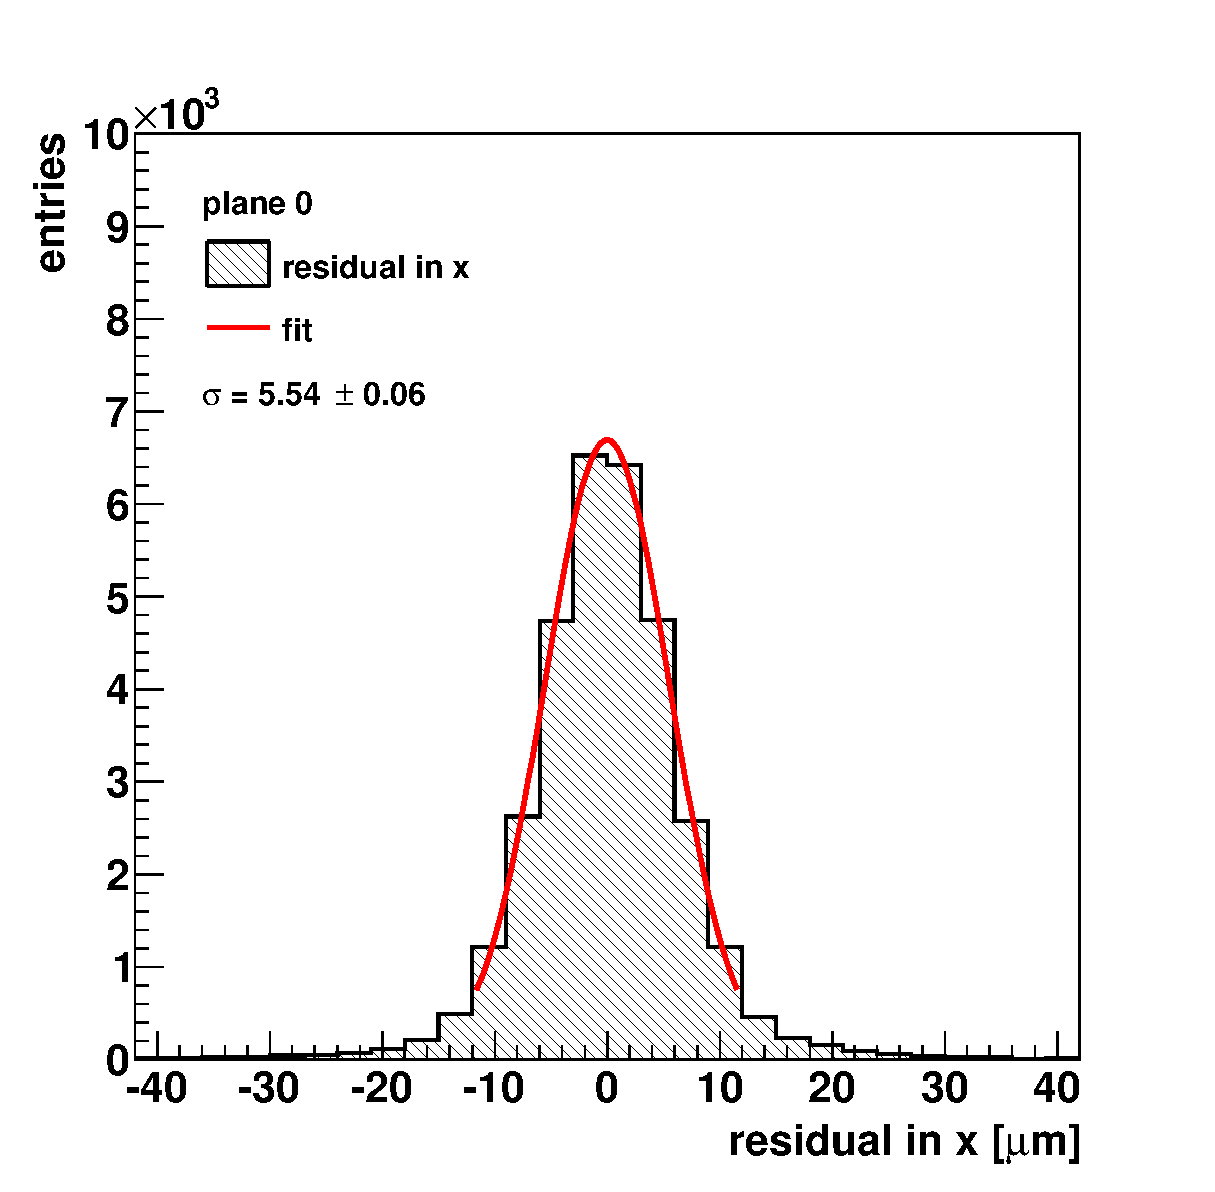
\includegraphics[width=0.49\textwidth]{figures/0x} \put(-50,155){(A)}
  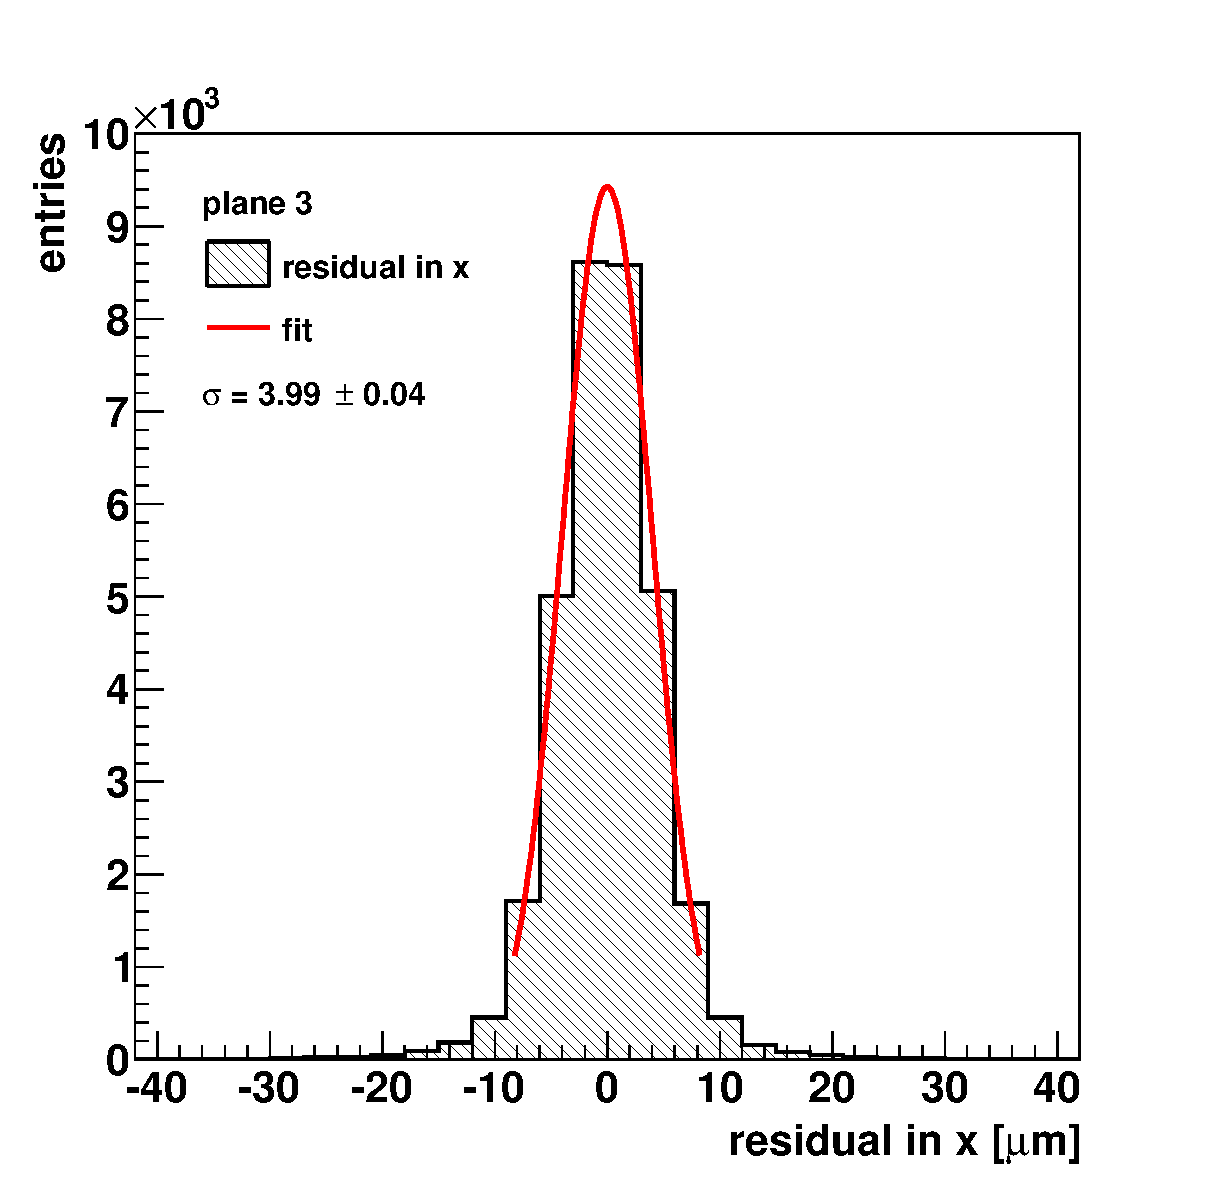
\includegraphics[width=0.49\textwidth]{figures/3x} \put(-50,155){(B)}\\
  %\includegraphics[width=0.45\textwidth]{figures/resis_upstream/1x.pdf}
  %\includegraphics[width=0.45\textwidth]{figures/resis_upstream/1y.pdf}
  %\includegraphics[width=0.45\textwidth]{figures/resis_upstream/2x.pdf}
  %\includegraphics[width=0.45\textwidth]{figures/resis_upstream/2y.pdf}
  %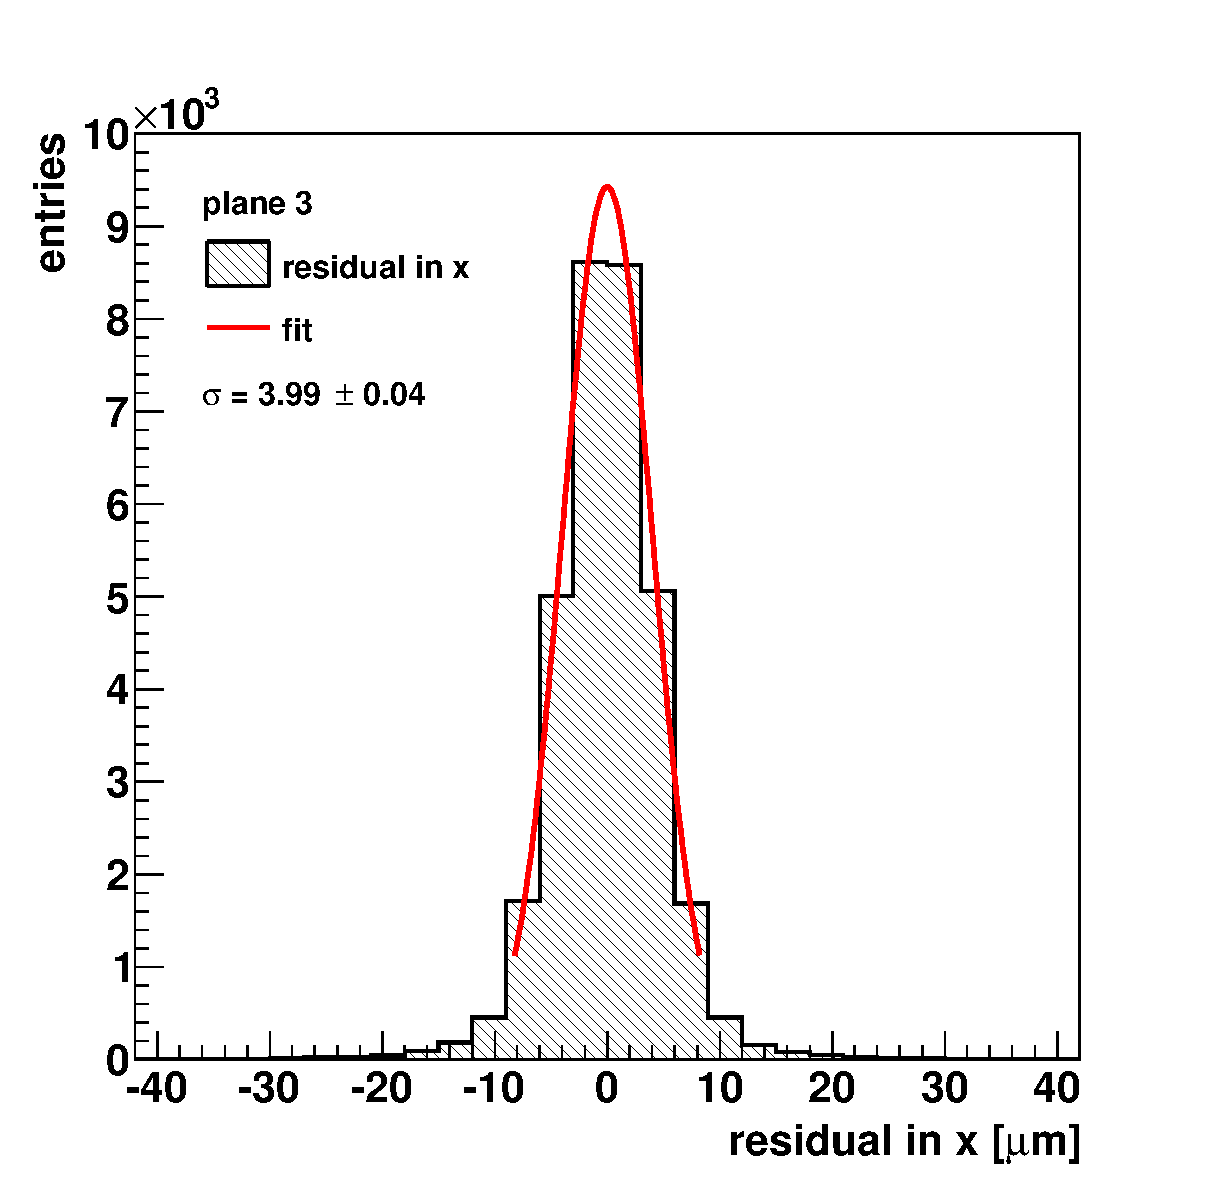
\includegraphics[width=0.49\textwidth]{figures/3x} \put(-50,155){(C)}
  %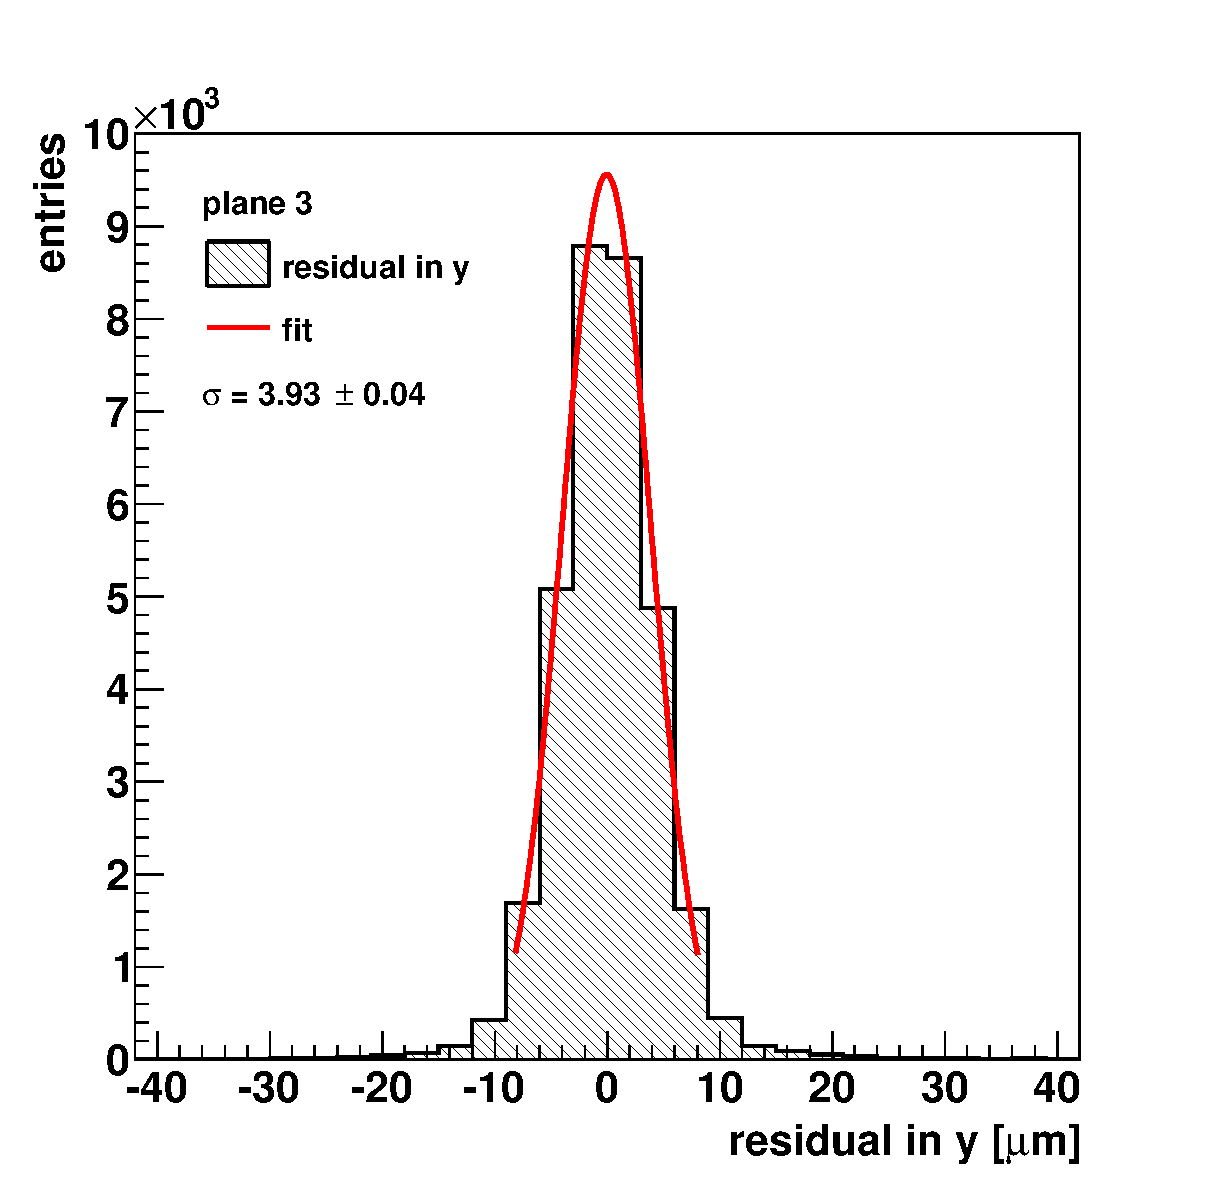
\includegraphics[width=0.49\textwidth]{figures/3y} \put(-50,155){(D)}
  %\includegraphics[width=0.45\textwidth]{figures/resis_downstream/4x.pdf}
  %\includegraphics[width=0.45\textwidth]{figures/resis_downstream/4y.pdf}
  %\includegraphics[width=0.45\textwidth]{figures/resis_downstream/5x.pdf}
  %\includegraphics[width=0.45\textwidth]{figures/resis_downstream/5y.pdf}
  \caption[Residual examples to determine the $\Datura$ telescope's resolution~\cite{ref:thomas}]{
  Unbiased residual distributions measured with the $\Datura$ telescope.
  The measured residuals in the $x$-direction for plane $0$ (A) and plane $3$ (B) are shown.
  According results in the $y$-direction and further planes are omitted. (reproduced from~\cite{ref:thomas})}
  \label{fig:residualexample1}
\end{figure}

\noindent
with $k_5$ being the geometrical scaling factor for a telescope consisting of five planes. 
The value of $k_5$ depends on the geometry itself and on which telescope plane is considered as DUT. 
Figure~\ref{fig:residualexample1} shows an example of unbiased residual distributions for a telescope sensor spacing of $\dz = 20\,\milli\meter$,
 a beam energy of $5\,\giga\electronvolt$, and a sensor threshold setting of $\noise = 6$.
The distributions are fitted with a Gaussian, from which the residual width $\sigma_{\textrm{meas}}$ is determined. 
For plane $3$, the residual width averaged over the $x$- and $y$-direction is $\left( 3.96\,\pm\, \allowbreak 0.03 \right)\,\micro\meter$. 
It is noted, that the residuals feature non-Gaussian tails, as is expected from the underlying physics of the scattering mechanism~\cite{ref:PDG-2014}. 
The measured resolution used in this work is defined as the width of a Gaussian fit on the centre $90\,\%$ of the residuals. 
The residual width for the outer plane $0$ is larger than the width obtained from plane $3$.
This is expected due to the fact that the track extrapolation to the inner sensors is done from both sides, hence is comparatively more precise than for the outer sensors,
 where the extrapolation can only be performed from one direction. 






% \begin{figure}[hbtp]
% \centering
% 
% \caption[Residual examples to determine the DATURA telescope's
% resolution. Downstream lever arm]{Residual examples to determine the DATURA
% telescope's resolution from the downstream lever arm. From top to bottom: The
% measured residuals for planes $3$, $4$ and $5$, left for $X$ direction, right
% for $Y$ direction. Each sensor plane was considered as a passive layer during
% the track reconstruction.}
% \label{fig:residualexample2}
% \end{figure}

By employing a $\chi^{2}$-minimisation method~\cite{ref:eudetmemo_2007_01,ref:lutzpaper}, the intrinsic resolution of the $\Mimosa$ sensors is calculated from the unbiased residual widths.
For each telescope sensor dimension ($x$- and $y$), the individual contribution $\Delta \chi^2_{i}$ from plane $i$ is defined as

\begin{equation}
\label{eq:chi2contrib}
\Delta \chi^2_{i} = \left( \frac{r - p_{i}}{\sigmai} \right)^2 \Bigg|_{i \ne i_{\textrm{DUT}}} +
\left( \frac{\theta_{\textrm{i}} - \theta_{i-1}}{\Theta_{0}} \right)^2 \Bigg|_{i \ne 0,N-1} \,,
\end{equation}

\noindent
with the telescope plane numbering beginning at zero.
The measured hit position on one dimension is denoted by $r$, the position extrapolated from the track in the same dimension by $p_{i}$.
The angles between the nominal beam direction and the track direction are $\theta_{i-1}$ and $\theta_{i}$.
The former is the track angle entering plane $i$, the latter the angle of the outbound track segment.
$\sigmai$ and $\Theta_{0}$ are the intrinsic resolution of sensor plane $i$ and the width of the multiple scattering distribution, according to equation~(\ref{eq:multiplescattering}), respectively.
It is assumed that $\sigmai$ and $\Theta_{0}$ do not differ between planes and that $\sigmai$ is also equal for both measurement dimensions.
If the beam axis is denoted by $z$, then $\theta_i$ can be expressed as

\begin{equation}
\theta_i = \frac{p_{i+1} - p_i}{z_{i+1} - z_i} \,.
\end{equation}


In equation~(\ref{eq:chi2contrib}) the first term, resulting from the hit measurement, is excluded in the $\chi^2$ calculation if the considered plane is the DUT.
Similarly, for the first and last planes the second term in equation~(\ref{eq:chi2contrib}) is omitted, since the scattering angle can not be determined.
This results in the global $\chi^2$ expression:

\begin{equation}
\label{eq:globalchi2}
\chi^2 = \sum_{i=0}^{N} \alpha_i \left( r - p_i \right)^2 + \sum_{i=1}^{N-1}
\left( \frac{p_{i + 1} \beta_i + p_{i-1} \beta_{i-1} - p_i \left( \beta_i + \beta_{i-1} \right)}{\Theta_0} \right)^2 \,,
\end{equation}

\noindent
with coefficients $\alpha_i$ and $\beta_i$ defined as~\cite{ref:eudetmemo_2007_01}

\begin{equation}
\alpha_i = \left\{
  \begin{array}{l l}
    \sigma_{i}^{-2} & \quad \text{for $i \neq i_{\textrm{DUT}}$}\\
    0 & \quad \text{for $i = i_{\textrm{DUT}}$}
  \end{array} \right. \quad \text{and} \quad \beta_i = \frac{1}{z_{i + 1} - z_i} \,.
\end{equation}

\begin{figure}[tbp]
  \centering
  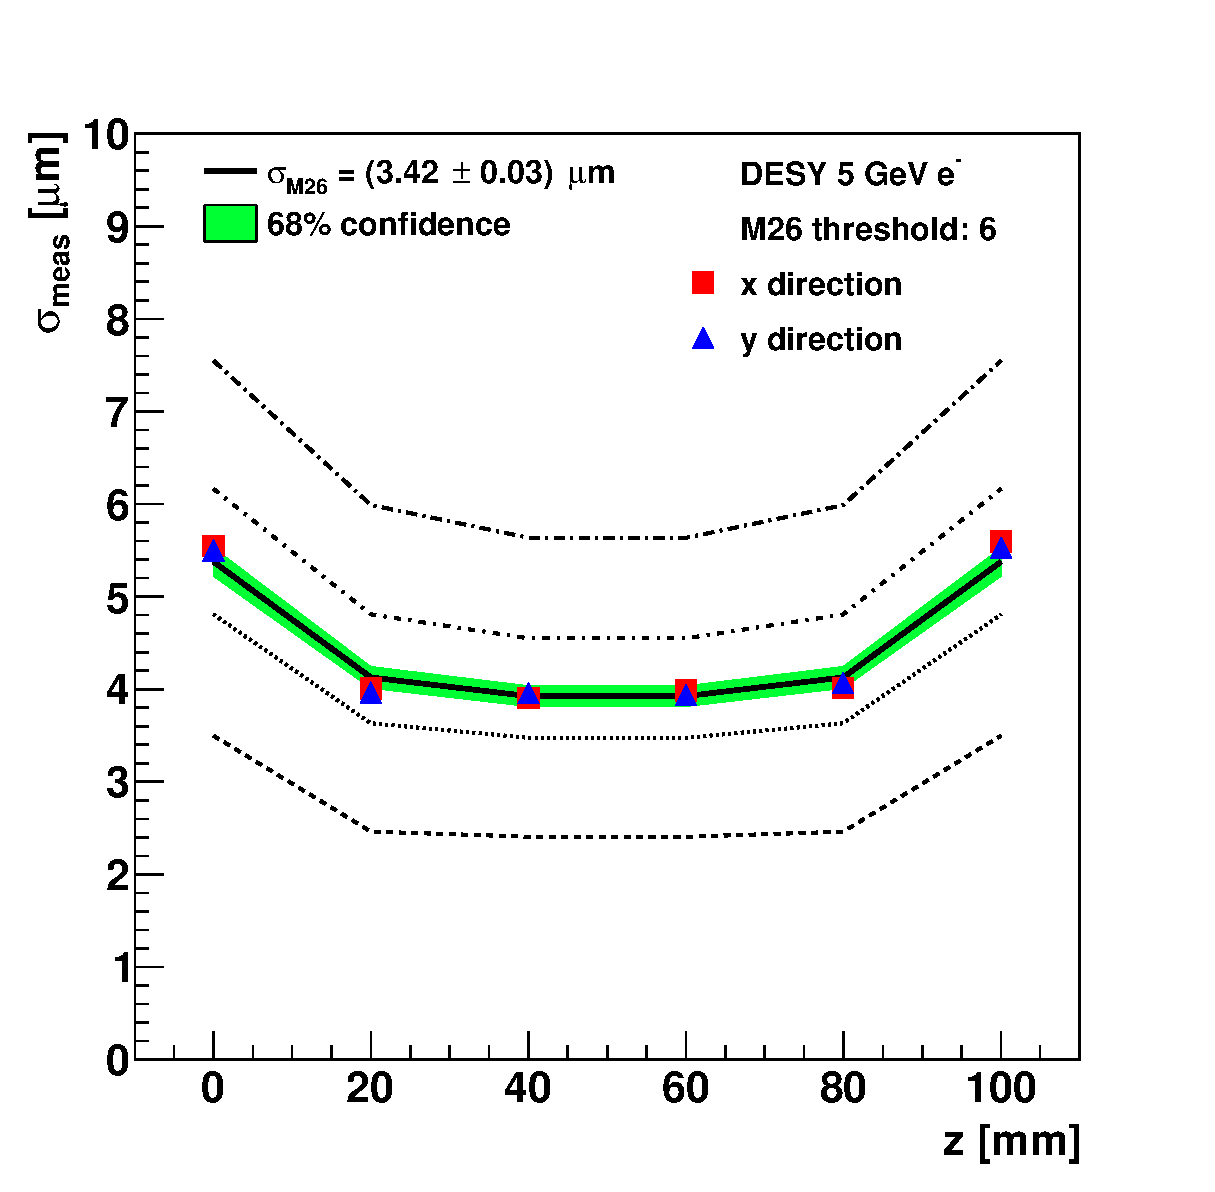
\includegraphics[width=0.49\textwidth]{figures/20}  \put(-50,40){(A)} % was thin_smiley.pdf
  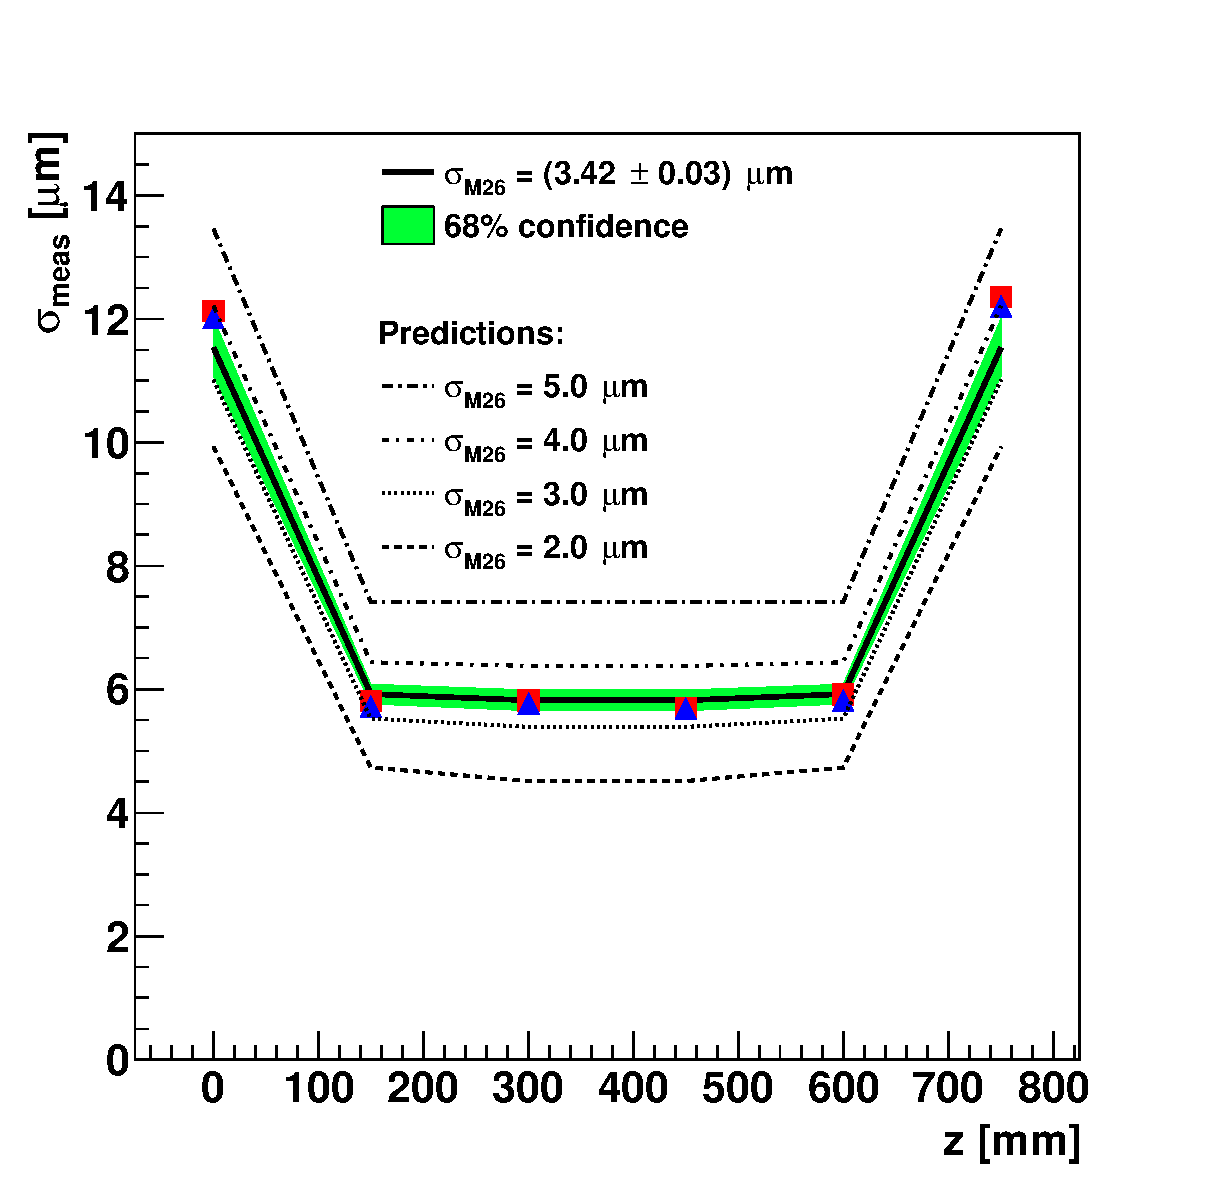
\includegraphics[width=0.49\textwidth]{figures/150} \put(-50,40){(B)} % was wide_smiley.pdf
  %\caption[Intrinsic telescope sensor resolution at $20\,\milli\meter$ and $150\,\milli\meter$ plane spacing~\cite{ref:thomas}]{Intrinsic telescope sensor resolution at $20\,\milli\meter$ (top)
  % and $150\,\milli\meter$ (bottom) plane spacing.
  \caption[The measured residual widths of each telescope plane.]{
  The measured residual widths of each telescope plane are shown in both the $x$- and $y$-direction for a plane spacing of $\dz = 20\,\milli\meter$ (A) and $\dz = 150\,\milli\meter$ (B).
  The black line shows the predicted residual width at $\sigmames = 3.43\,\upmu\meter$, the green band the measurement standard deviation.
  Dotted and dashed lines indicate the predicted residuals width, in case differing intrinsic resolutions are assumed.
  Data was taken at a sensor threshold of $\noise = 6$ and using $5\,\giga\electronvolt$ electrons at DESY-II.
  (reproduced from~\cite{ref:thomas})}
  \label{fig:smiley}
\end{figure}

\noindent
The minimum of equation~(\ref{eq:globalchi2}) is then calculated to find the intrinsic sensor resolution $\sigmai$.
The results for both a tighter plane spacing of $\dz = 20\,\milli\meter$ and a wider spacing of $dz = 150\,\milli\meter$ are shown in figure~\ref{fig:smiley}.
In both cases, an error of $0.5\,\milli\meter$ on the plane distance $\textrm{d}z$ is assumed.
The calculated intrinsic resolution $\sigma_{\textrm{M26}} = \sigmai$ of the $\Mimosa$ sensors is \allowbreak$\left( 3.42\,\pm\, \allowbreak 0.03 \right)\,\micro\meter$
 for a plane spacing of $\textrm{d}z =  20\,\milli\meter$ and $\left( 3.44\,\pm\, \allowbreak 0.03 \right)\,\micro\meter$ for $\textrm{d}z = 150\,\milli\meter$. 
The average over the two configurations results in $\sigma_{\textrm{M26}} = \left( 3.43\,\pm\, \allowbreak 0.03 \right)\,\micro\meter$. 
The stated uncertainty is the error on the mean, the standard deviation is $0.10\,\micro\meter$.
For both geometries, the expected resolution of $\sigmai \approx\,3.5\,\micro\meter$~\cite{ref:mimosa26} can be confirmed.
The underlying assumptions in the above method are:

\begin{itemize}

\item The multiple scattering terms described in equation~(\ref{eq:telescoperesolutionequation_2}) are calculated considering the nominal sensor thicknesses, the air between sensor planes, and a $25\,\micro\meter$
thick Kapton foil on either side of each sensor.
In the multiple scattering term $\sigma_{\textrm{MS}}$, the nominal beam energy is used. 

\item The intrinsic resolution $\sigmai$ of all sensor planes is assumed to be equal.
As the discriminator thresholds are set for subframes of each plane individually, this is not necessarily true.
%Figure~\ref{fig:resivsenergy_thresh} shows the dependence of $\sigmai$ on the applied SNR threshold.

\end{itemize}

%\item Residual widths are calculated using straight line tracks only.
%Inclined tracks, or a deflection of tracks in planes or scattering material, are not taken into account.
%However, as shown in~\cite{ref:lutzpaper}, angular deflections are then considered for the later $\chi^2$ minimisation.

Furthermore, the above described method has been repeated for various sensor thresholds, each resulting in an estimate for $\sigmai$ as a function of the set threshold $\noise$. 
Figure~\ref{fig:resivsenergy_thresh} (A) shows the intrinsic sensor resolutions $\sigmai$ derived from the measurements for different beam energies and plane distances as a function of the applied sensor threshold.
The minimum of $\sigmai$ is reached for a threshold setting of $\noise = 6$.
The measured residual width for the wider sensor spacing or lower beam energies is higher as can be seen in figure~\ref{fig:smiley}.
These effects are described in equation~(\ref{eq:telescoperesolutionequation}) by the terms $\sigma_{\textrm{Tel}}^2$ and $\sigma_{\textrm{MS}}^2$.
Previous measurements~\cite{ref:j.behrmeasurements} taken at $\noise\,>\,10$ show comparable results of $\sigma_{\textrm{M26}} = (4.35\,\pm\,0.10)\,\micro\meter$.
%Measurements by Behr~\cite{ref:j.behrmeasurements} taken at $\noise\,>\,10$ show comparable results of $\sigma_{\textrm{M26}} = (4.35\,\pm\,0.10)\,\micro\meter$.
% If Joerg is on the author list, rephrase the citation...

% Thomas: sigma tel is different from the pointing resolution.
% leave this out as to not confuse reader.
%From equation~(\ref{eq:telescopepointing}) the optimal track pointing resolution $\sigma_{\textrm{Tel}}$ of the $\Datura$ telescope without multiple scattering
% can therefore be given as $\left( 1.40 \pm 0.05 \right)\,\micro\meter$.


\begin{figure}[tbp]
  \centering
  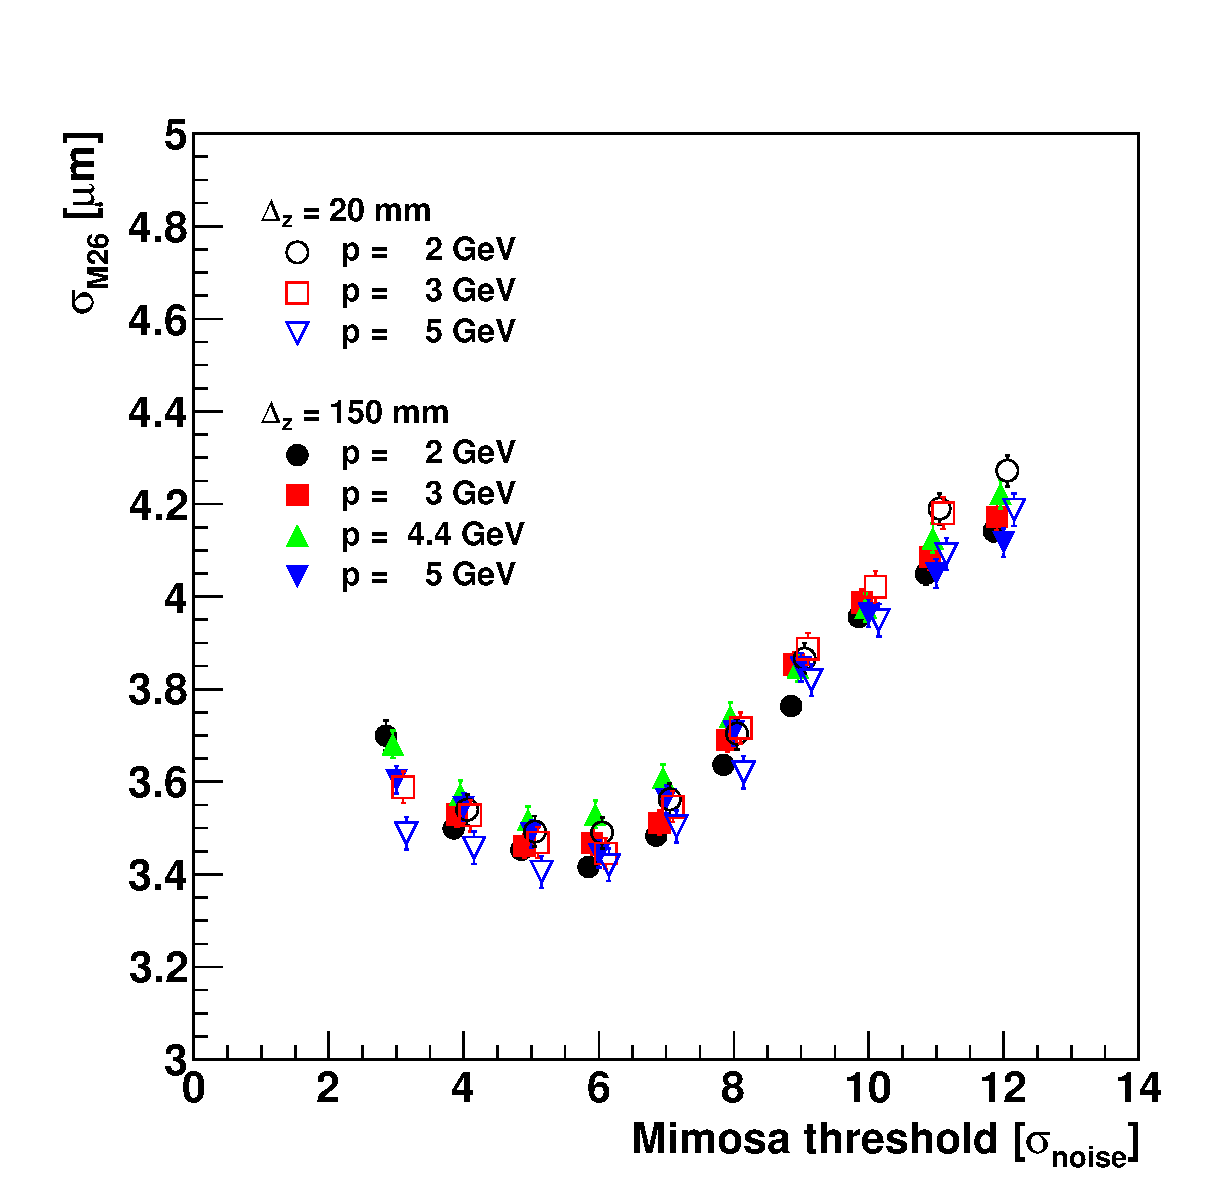
\includegraphics[width=0.49\textwidth]{figures/resi_vs_thresh}	\put(-40,35){(A)} % was resi_thresh_errors
  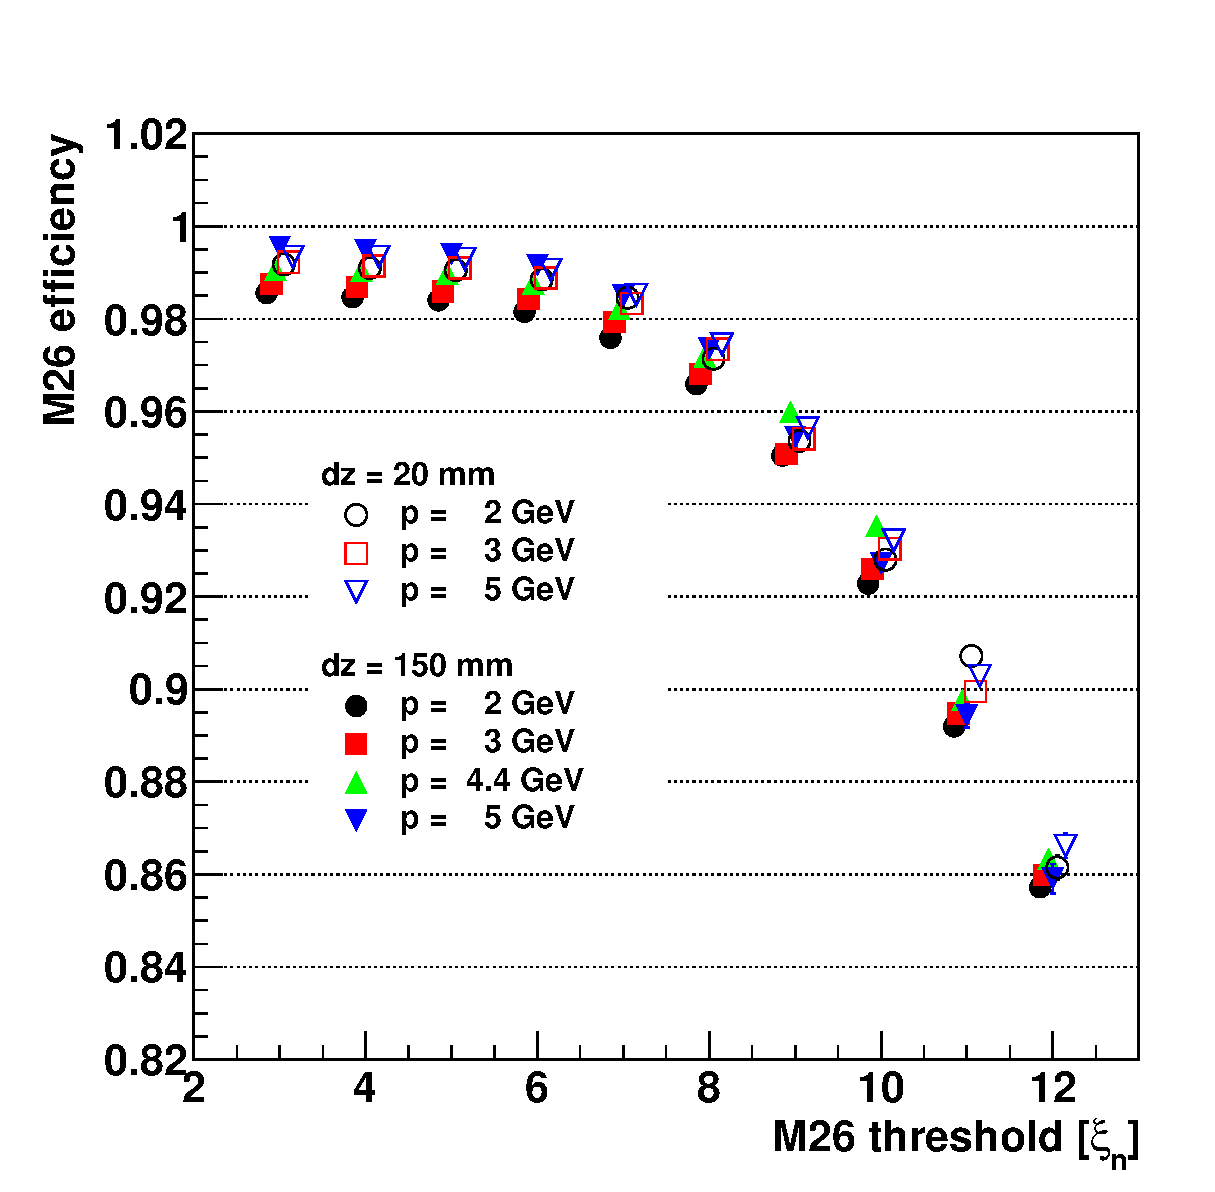
\includegraphics[width=0.49\textwidth]{figures/effi_thresh.eps}	\put(-175,35){(B)}
  \caption[Telescope intrinsic sensor resolution for different threshold settings, beam energies and geometries~\cite{ref:thomas}]{
(A) The measured intrinsic resolution of the $\sigma_{\textrm{M26}}$ for different beam energies $p$ and sensor spacing $\textrm{d}z$ as a function of the applied sensor threshold $\noise$.
(B) Average efficiency of all telescope sensors for different beam energies and sensor spacing vs.~applied threshold.
An efficiency decline with increasing threshold can be observed.
In both images values are shifted on the $x$-axis for improved legibility.
(reproduced from~\cite{ref:thomas})}
  \label{fig:resivsenergy_thresh}
\end{figure}

The threshold applied to each telescope sensor is a critical parameter for the telescope performance.
A higher threshold cuts into the signal, reducing the amount of clusters found on each plane and thus limiting the number of reconstructible tracks.
This reduces the sensor efficiency.
A lower threshold allows for an increasing number of noise induced signals to pass the zero-supression on the chip.
This leads to a broadening of the residual distributions and hence a worse resolution. 
%Figure~\ref{fig:effi} shows the efficiency distribution over a sensor plane.
The efficiency is defined as the ratio of reconstructed tracks that have at least one hit on the DUT within $100\,\micro\meter$ to the overall number of tracks.
%As maximum distance $100\,\micro\meter$ is considered.
%A noisy pixel column at $Y \approx -8\,\milli\meter$ can be observed.
%This column was masked during the converter step in the \texttt{datura-noDUT} example and subsequently is not used during the analysis. 
%\\{comment hj: datura-noDUT is jargon}
%Disregarding this area, an overall average efficiency over $98\,\%$ is observed.
In figure~\ref{fig:resivsenergy_thresh}~(B) the efficiency dependence on the sensor threshold is shown for various beam energies and sensor spacings.
Efficiencies are averaged over all six sensor planes and both spatial coordinates, resulting in negligible statistical errors. 
In all cases, the efficiency is above $98\,\%$ up to a threshold of $7$.
With increasing threshold, the efficiency declines until a level of $86\,\%$ at $\noise = 12$ is reached.
The difference in efficiency for different energies and for different plane spacings stems from multiple scattering and different extrapolation lengths due to differing $\dz$.

%\begin{figure}[tbp]
%  \centering
%  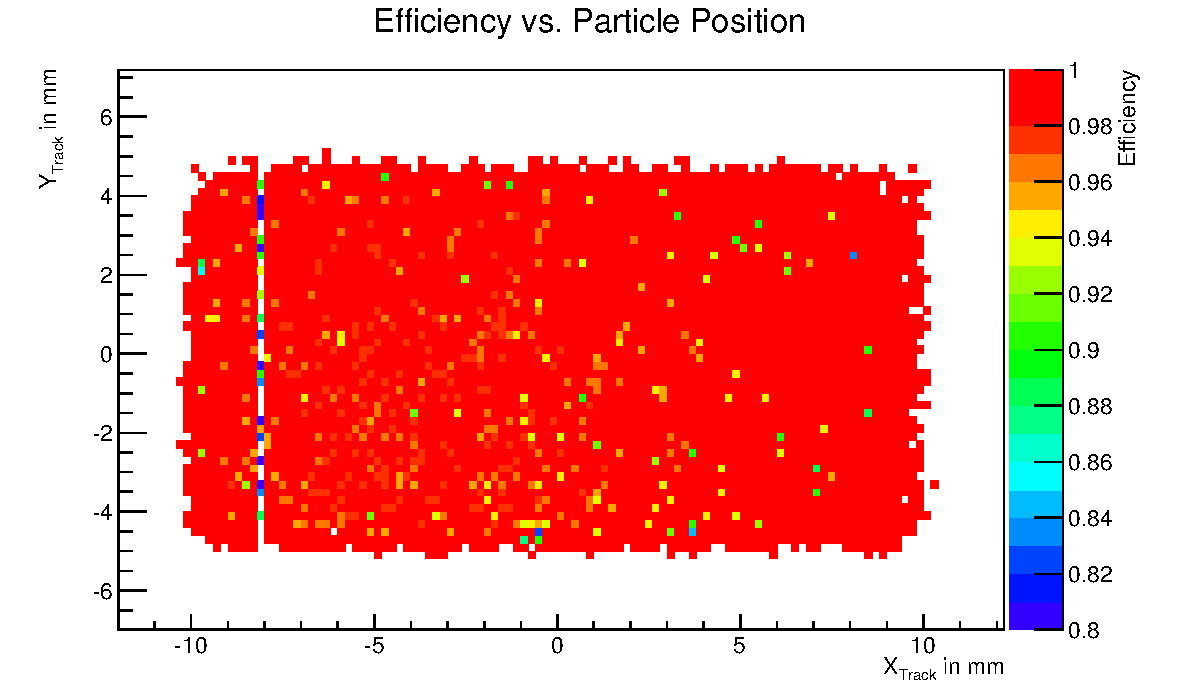
\includegraphics[width=\textwidth]{figures/plane3_effi_run37.pdf}
%  \caption[Telescope sensor efficiency~\cite{ref:thomas}]{Efficiency of telescope sensor plane $3$ at a threshold of $7$ and $5\,\giga\electronvolt$ beam momentum.
%Image from~\cite{ref:thomas}.}
%\label{fig:effi}
%\end{figure}



%\begin{figure}[tbp]
%  \centering
%  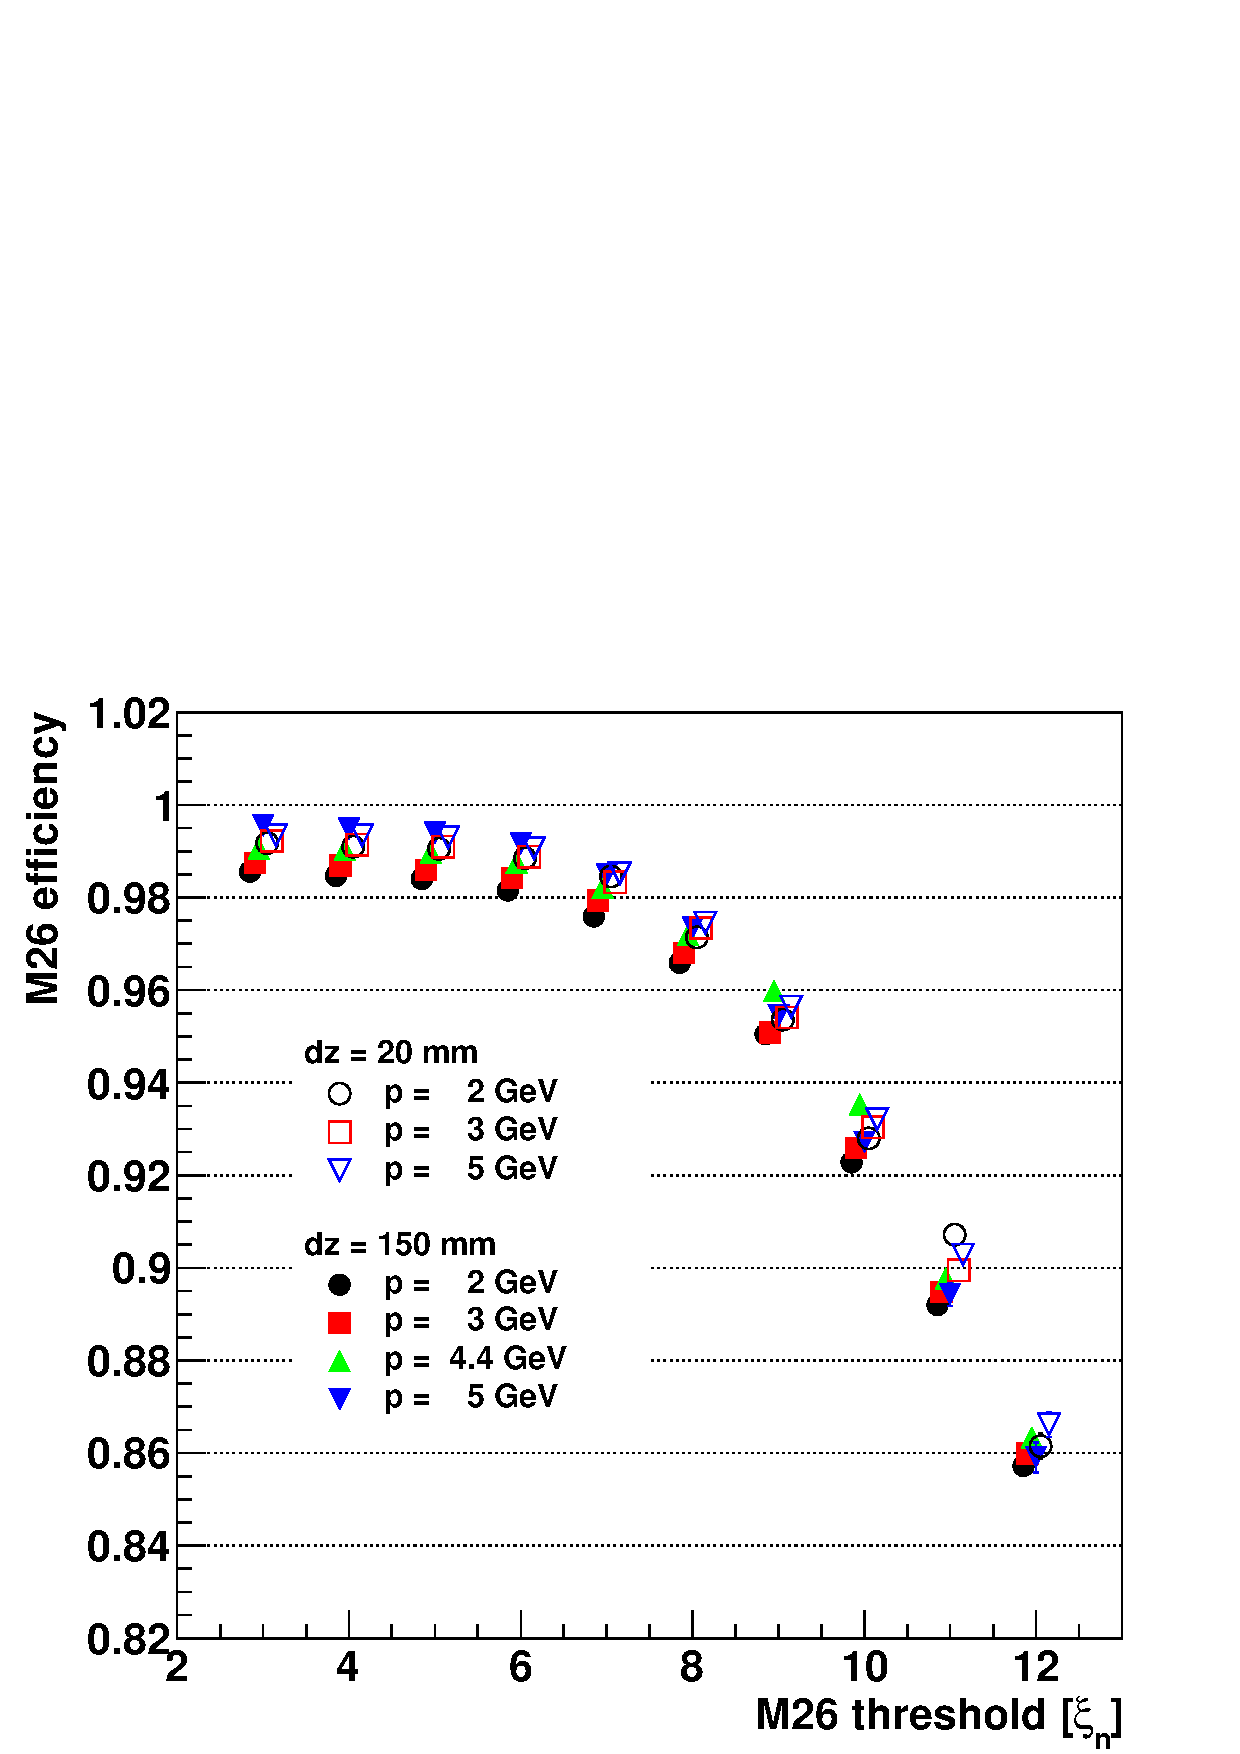
\includegraphics[width=\textwidth]{figures/effi_thresh.pdf}
%  \caption[Overall telescope sensor efficiency vs. threshold for different beam momenta and sensor spacings~\cite{ref:thomas}]{
%Average efficiency of all telescope sensors in both dimensions for different beam momenta and sensor spacing vs. applied threshold.
%An efficiency decline with increasing threshold can be observed.
%Some values are shifted on the $x$ axis for improved legibility.
%Image from~\cite{ref:thomas}.}
%\label{fig:effi_thresh}
%\end{figure}



\subsection{Resolution predictions using General Broken Lines}

Using the measured intrinsic resolution, the known material budget $\epsmimo = 7.1\cdot 10^{-4}$ of the sensor planes, and the material budget of the DUT $\epsdut$,
 predictions of the expected pointing resolution at the actual DUT position can be made. 
Therefore, it is possible to perform an a priori calculation of the optimal telescope geometry for a certain measurement set-up. 
Pointing resolutions in this section refer to the achievable pointing resolution using a \textit{symmetric six M26 planes plus DUT} configuration. 
This is referred to as \textit{user configuration}, also shown in figure~\ref{fig:datura_sketch}, while the set-up used in section~\ref{sec:measurements} is referred to as \textit{gauge configuration}. 

Using the GBL~\cite{Blobel20111760,Kleinwort-2012} formalism, the pointing resolution is analytically calculated at desired points of interest along the particle trajectory. 
The pointing resolution at the DUT for four different DUT material budgets $\epsdut$ is plotted as a function of the spacing $\dzdut$ in figure~\ref{fig:CalcResos_dzdut}.
Exemplified are two values of $\dz = 20\,\milli\meter$ and $\dz = 50\,\milli\meter$. 
Plots are provided for DESY-II beam energies (A) and SPS energies (B). 
All plotted resolution functions monotonically increase with increasing $\dzdut$. 
To achieve the best possible resolution, the inner $\Mimosa$ planes should be positioned as close as possible to the DUT, i.e.~$\dzdut$ is to be minimised. 
In addition, figure~\ref{fig:CalcResos_dzdut} shows, that the optimal plane spacing $\dz$ depends on the actual DUT material budget.
For instance for a DUT with a material budget of $\epsdut = 0.001$ (black and red solid lines) at 5\,GeV, a narrow configuration shows a higher resolution for $\dzdut < 70\,\milli\meter$,
 while a wide configuration is best for $\dzdut > 70\,\milli\meter$.
The position of the intersection of the the lines depends on the material budget of the DUT $\epsdut$ and decreases with increasing material budget. 
In the wide configuration, the predicted pointing resolution on the DUT is limited to about $2.3\,\upmu\meter$,
 whereas in a narrow configuration a pointing resolution of around $2.0\,\upmu\meter$ is achievable for thin DUTs.
At SPS energies, the resolution functions for the wide and the narrow configuration do not intersect, with the narrow configuration performing slightly better than the wide one.
However, the difference is less than $500\,\nano\meter$ for $\dzdut = 100\,\milli\meter$ even for $\epsdut = 0.03$. 

\begin{figure}[tbp]
  \centering
  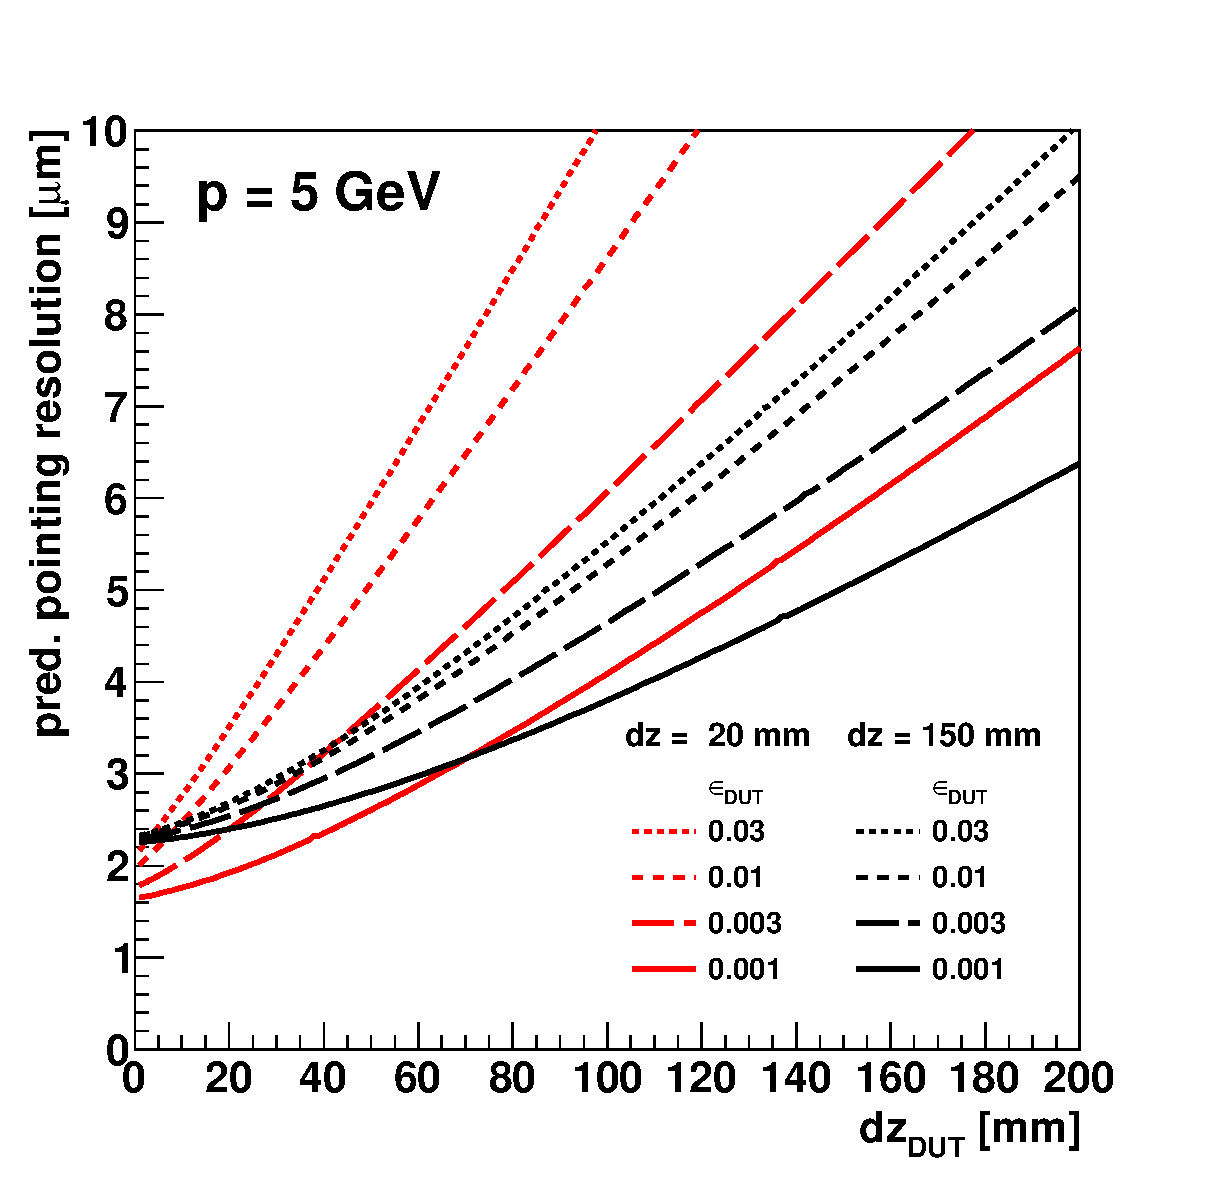
\includegraphics[width=0.49\textwidth]{figures/CalcResoVsDzdut_Desy}\put(-185,35){(A)}
  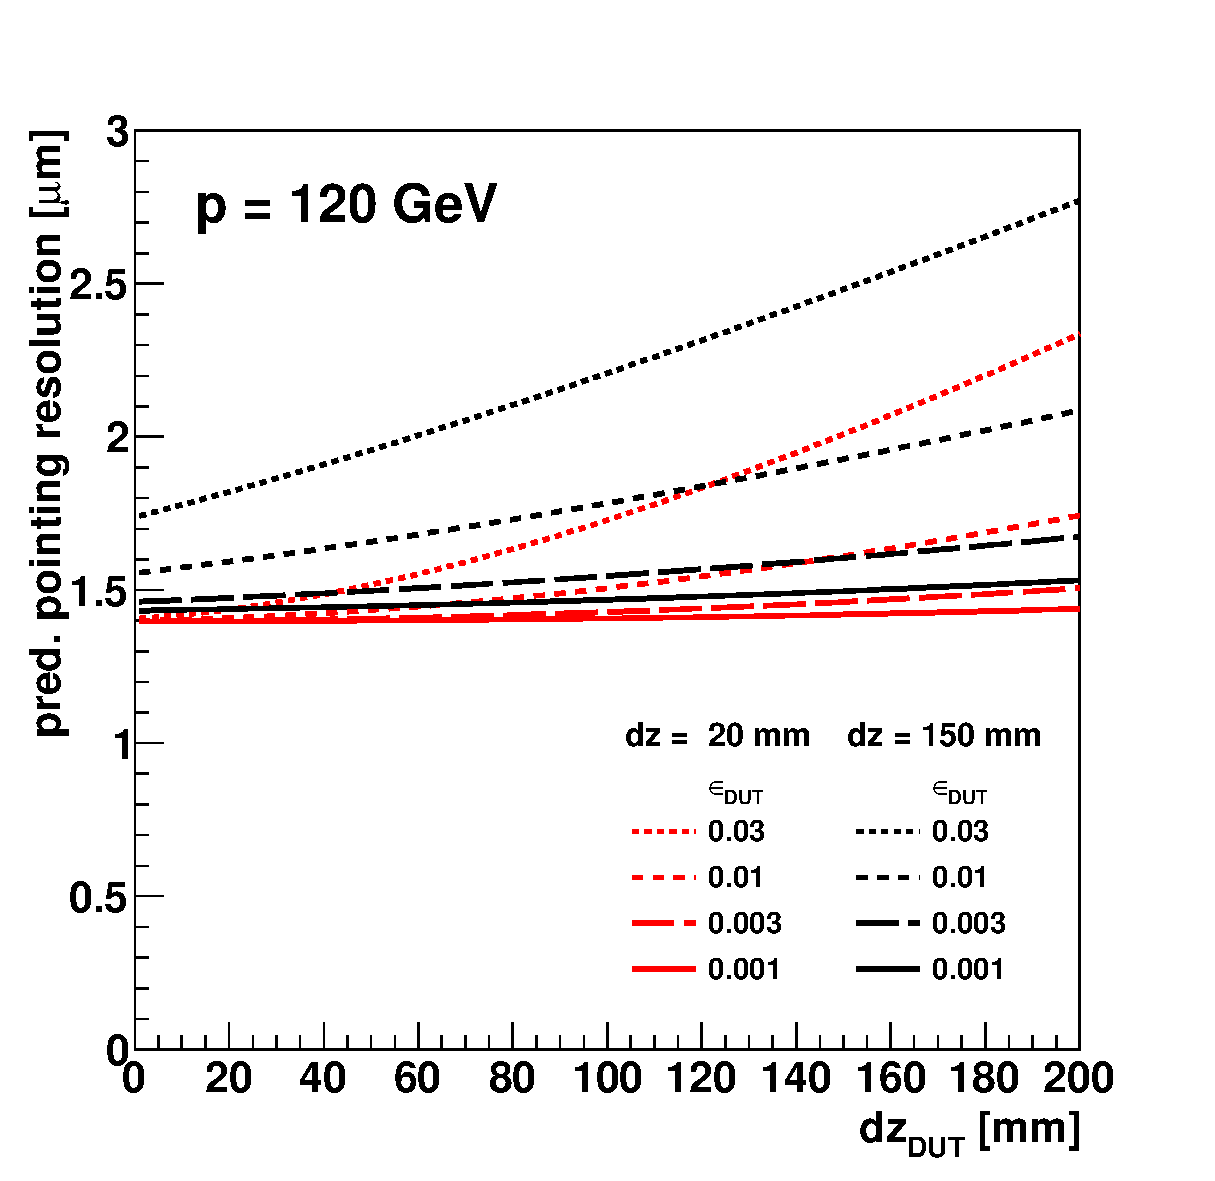
\includegraphics[width=0.49\textwidth]{figures/CalcResoVsDzdut_Cern}\put(-185,35){(B)}
  %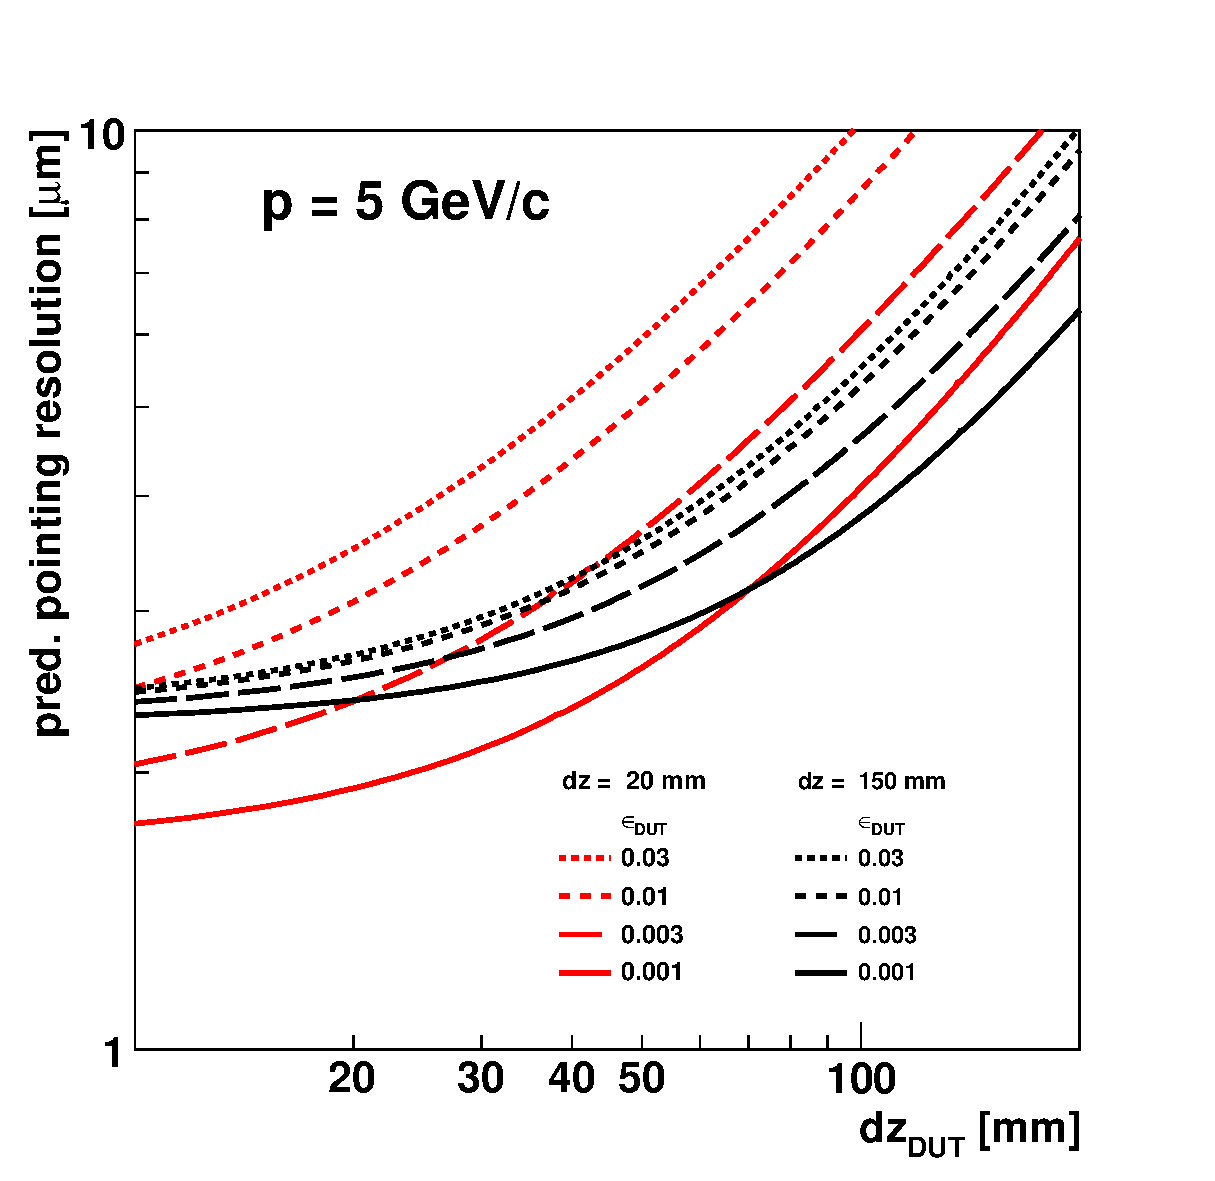
\includegraphics[width=0.49\textwidth]{figures/CalcResoVsDzdut_Desy_loglog_2}
  %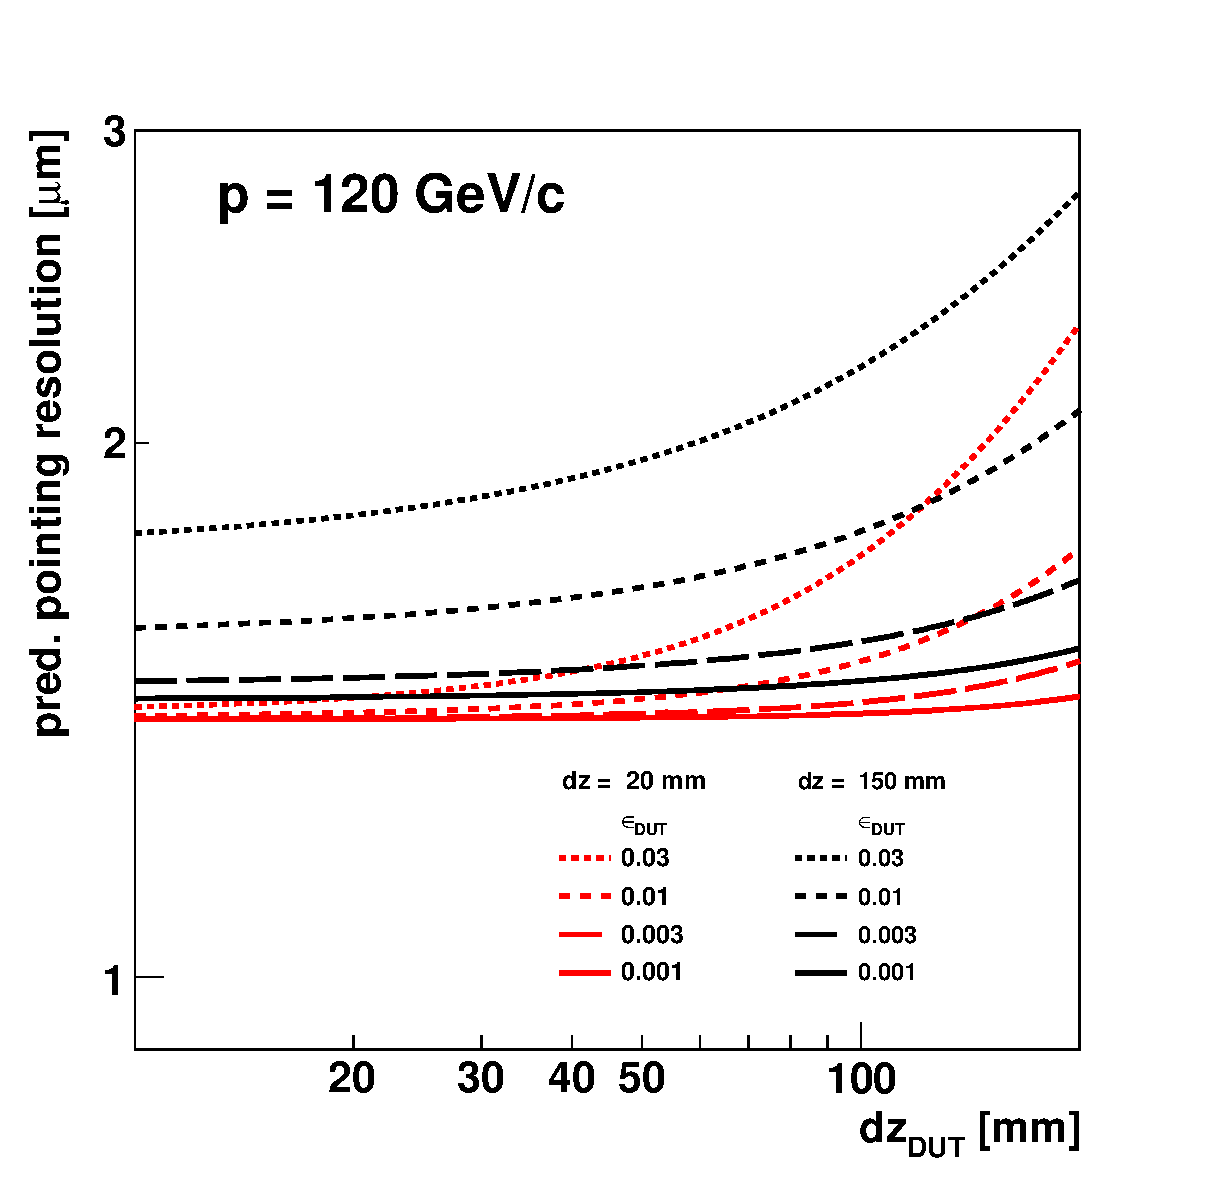
\includegraphics[width=0.49\textwidth]{figures/CalcResoVsDzdut_Cern_loglog_2}
  \caption[Pointing resolution for various material budgets as a function of the distance between DUT and neighbouring planes]{
  The pointing resolution for various material budgets is shown as a function of the equidistant spacing between DUT and neighbouring planes at 5\,GeV (A), and 120\,GeV (B) in the \textit{user configuration}.}
\label{fig:CalcResos_dzdut}
\end{figure}

Using the \textit{gauge configuration}, a comparison between the GBL calculations and the measurements can be performed.
For this, the measured resolution has to be converted to the pointing resolution $\sigmap$ by correcting for the intrinsic resolution of the DUT $\sigmadut = \sigmam$

\begin{equation}
 \sigmap = \sqrt{\sigmames^2 - \sigmadut^2}.
 \label{eq:sigmap}
\end{equation}

\noindent
This is shown in figure~\ref{fig:CalcResoP_DUT} (A) as a function of the beam energy. 
The solid lines represent GBL calculations, while the triangles show the derived $\sigmap$ obtained from equation~(\ref{eq:sigmap}). 
The hatched bands represent the calculated pointing resolution assuming $\sigmam = 3.43\,\upmu\meter$ with a standard deviation of $0.10\,\upmu\meter$ for the wide and the narrow configuration. 
An excellent agreement between GBL calculations and the measurements is found.

In figure~\ref{fig:CalcResoP_DUT} (B) the achievable pointing resolution as a function of the material budget is plotted for the \textit{user configuration}. 
It can be seen that a minimal $\dzdut$ allows for the best possible resolution. 
Dashed and solid lines represent calculations for $\dz = 20\,\milli\meter$ and $\dz = 150\,\milli\meter$, respectively. 
Their intersections mark the material budget, at which optimal plane spacing $\dz$ changes.
For $\epsdut$ below (above) the intersection, a narrow (wide) configuration is preferable. 
The position of the intersection shifts to smaller material budgets with increasing $\dzdut$. 

\begin{figure}[tbp]
  \centering
  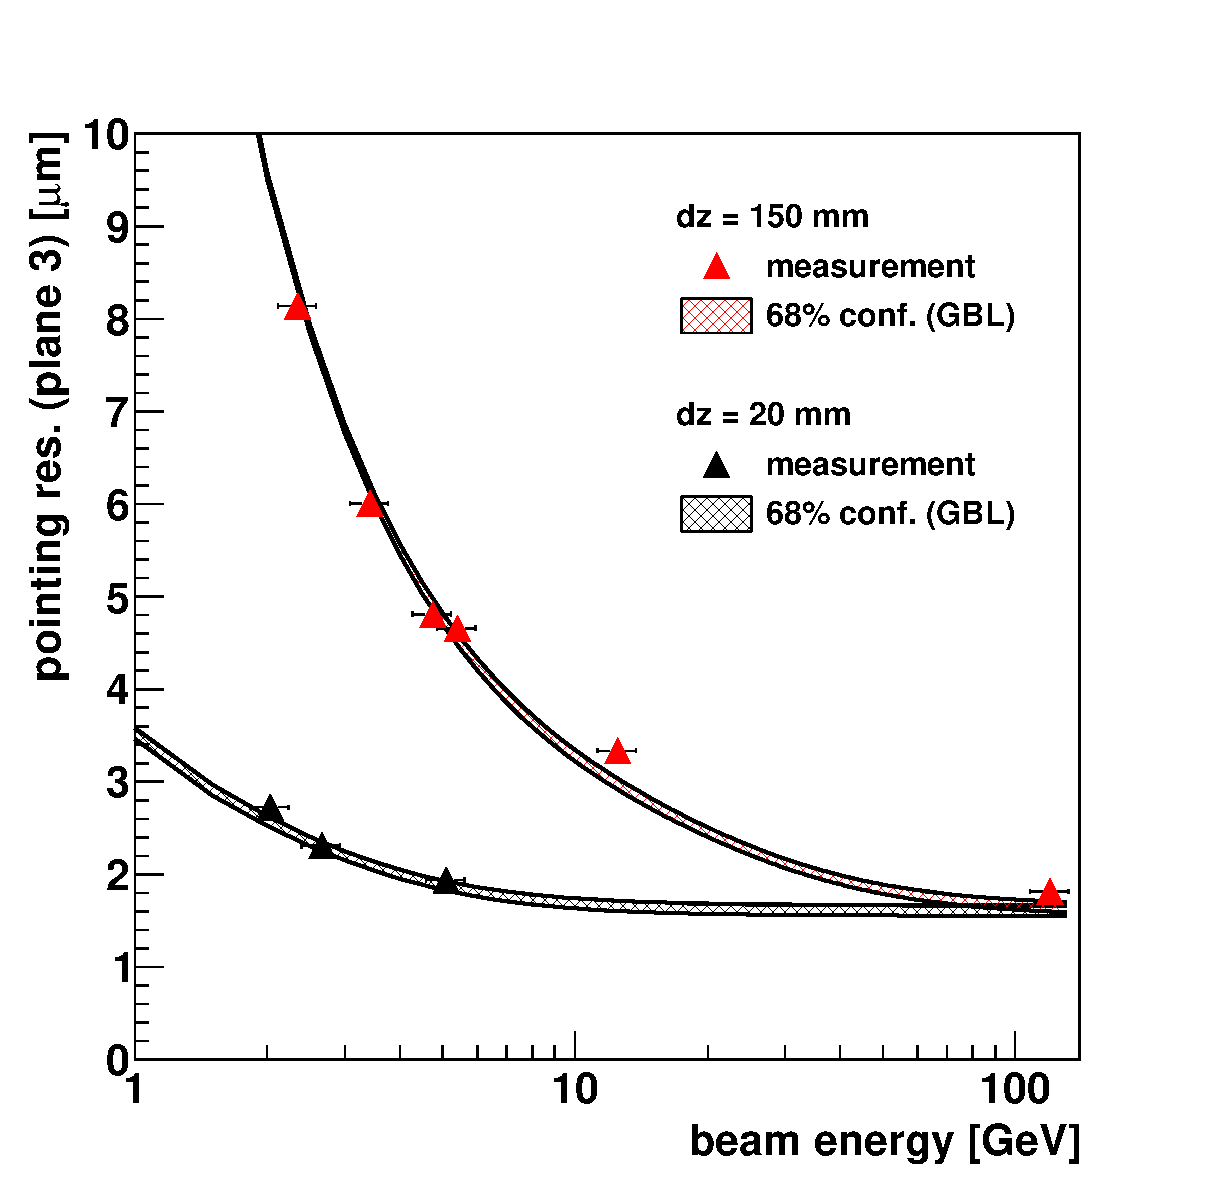
\includegraphics[width=0.49\textwidth]{figures/energy_plot}     \put(-175,40){(A)} % was CalcResoVsP
  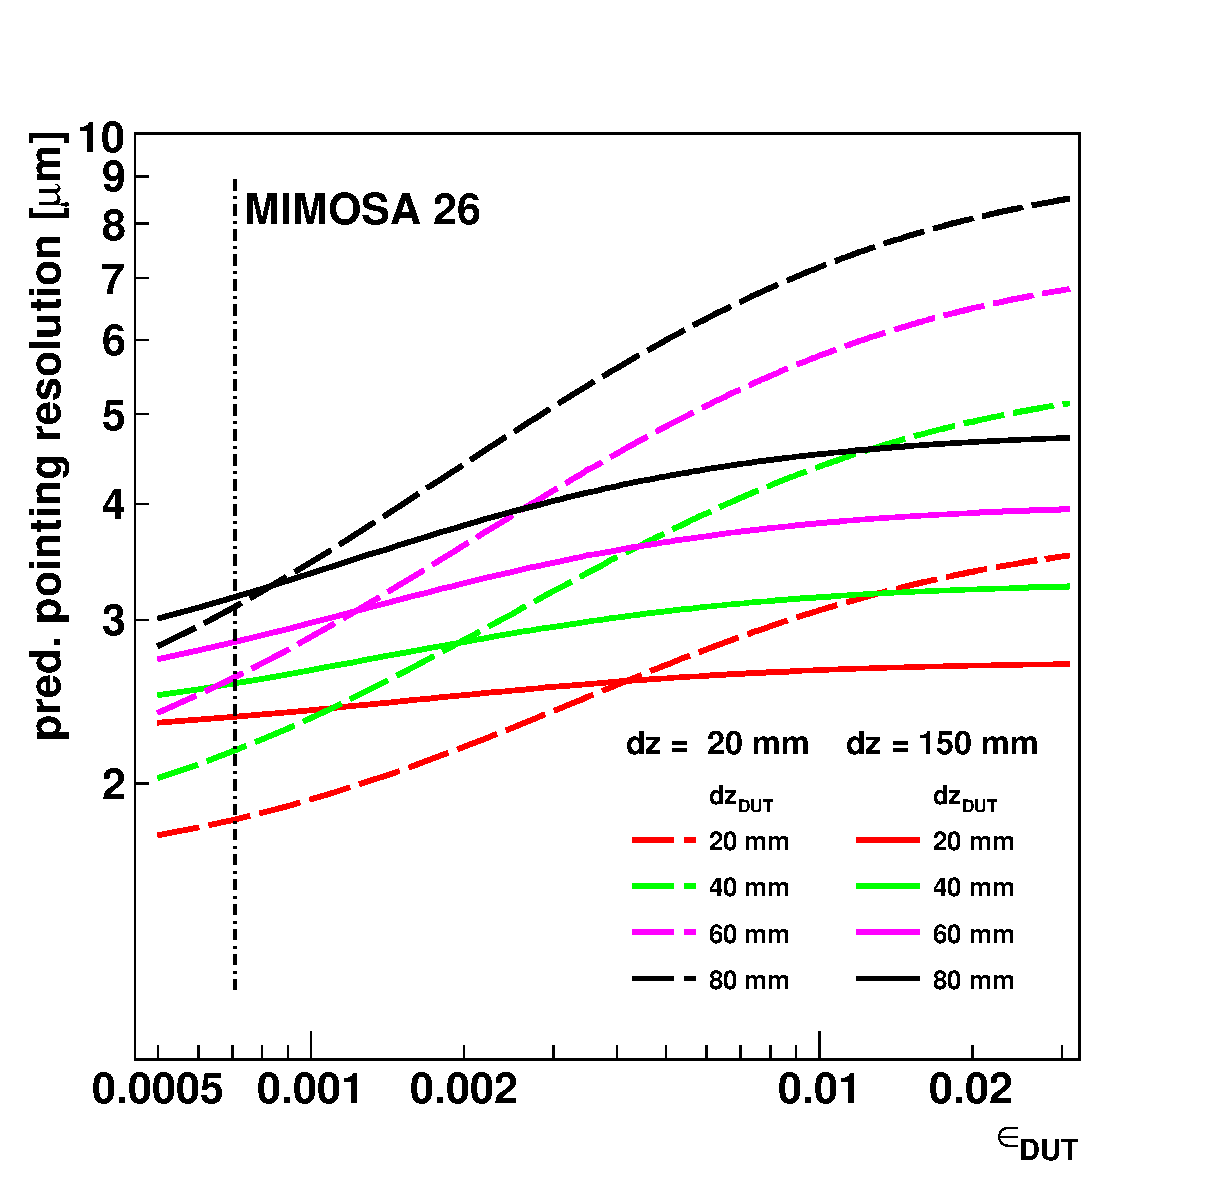
\includegraphics[width=0.49\textwidth]{figures/CalcResoVsEpsdut}\put(-155,40){(B)}
%               \put(-175,107.5){$\bigcirc$}
%  \color{blue} \put(-161,102.5){$\bigcirc$}
%  \color{green}\put(-143,96.5){$\bigcirc$}
%  \color{red}  \put(-113,90){$\bigcirc$}
%  \color{black}
   \caption[Pointing resolution as a function of the beam energy]{
   (A) The measured (triangles) and calculated (lines) pointing resolution at plane $3$
    for the wide (red) and the narrow (black) set-up is shown as a function of the beam energy for the \textit{gauge configuration}~\cite{ref:thomas}. 
   The solid lines form bands representing the standard deviation of $0.10\,\upmu\meter$ of the intrinsic resolution.
   %The theoretical limit of about $1.6\,\upmu\meter$ for plane\,3 is indicated as a dashed line.
   %Pointing resolutions derived from the measured resolutions at plane 3 for various energies and plane spacings are shown as crosses.
   (B) The calculated pointing resolutions at the DUT for two geometries are shown as a function of $\epsdut$ for the \textit{user configuration} at a beam energy of 5\,GeV.
   }
 \label{fig:CalcResoP_DUT}
\end{figure}
